\setlength{\tabcolsep}{1pt} % 默认值通常为6pt
\setlength{\topsep}{1pt}
\setlength{\partopsep}{1pt}
\setlength{\parskip}{1pt}

\section*{一、基本概念}

\subsection*{连续时间信号}

·\textbf{模拟信号}:时间幅值均连续;\textbf{数字信号}:时间幅值均离散;\textbf{采样信号}:时间离散幅值连续

·\textbf{能量(有限)信号}:$E= \int ^{\infty} _{-\infty} |f(t)|^2dt$(阶跃能量无穷大)

·\textbf{功率(有限)信号}:$P = \lim_{T\to\infty} \frac{1}{T} \int ^{\frac{T}{2}} _{-\frac{T}{2}} f(t)^2dt$

·\textbf{采样信号} $Sa(t) = \frac{\sin(t)}{t}$;偶函数;$t = \pm \pi, \pm 2 \pi, ...$时$Sa(t)=0$;
   $\int ^{\infty} _{-\infty} Sa(t)dt = \pi;\int ^{\infty} _{0} Sa(t)dt = \frac{\pi}{2}$;以$\frac{1}{t}$衰减

·\textbf{正余弦和指数}:$sin(\omega t)=\frac{1}{2j}(e^{j\omega t}-e^{-j\omega t})$;$cos(\omega t)=\frac{1}{2}(e^{j\omega t}+e^{-j\omega t})$

·\textbf{单位阶跃信号} $u(t)$,注意$u(0)=0.5$

·\textbf{单位斜变信号} $f(t) = tu(t)$

·\textbf{符号函数} $sgn(t) = 2u(t) - 1 = u(t) - u(-t)$

·\textbf{单位脉冲信号} $\delta (t) = \lim_{\tau\to0}\frac{1}{\tau}[u(t+\frac{\tau}{2})-u(t-\frac{\tau}{2})]$
   
   1. $\int ^{\infty} _{-\infty} \delta (t)dt = 1; \delta (t) = 0, t \ne 0$ 狄拉克(Dirac)定义
   
   2. $\int ^{\infty} _{-\infty} \delta (t-t_0)f(t)dt = f(t_0)$【$\delta (t)f(t) = \delta(t)f(0)$】
   
   3. 偶函数$\delta(t) = \delta(-t);$导数为奇函数$\delta'(t) = -\delta'(-t)$
   
   5. $u(t)=\int ^t _{-\infty} \delta(\tau)d\tau; \int ^{\infty} _{0} \delta(t-\sigma)d\sigma = u(t)$
   
   6. $\delta(at) = \frac{1}{|a|}\delta(t)$
   
   7. $\delta'(t)=\lim_{\tau\to0}\frac{1}{\tau}[\delta(t+\frac{\tau}{2})-\delta(t-\frac{\tau}{2})]=\frac{d\delta(t)}{dt}$ 
   
   8. $\delta'(0_-) = + \infty ; \delta'(0_+) = - \infty$
   
   9. $\int ^{\infty} _{-\infty} \delta' (t)dt = 0; \delta(t)=\int ^t _{-\infty} \delta'(\tau)d\tau$
   
   10. $\int ^{\infty} _{-\infty} \delta' (t-t_0)f(t)dt = -f'(t_0)$ 抽样特性
   
   11. $\delta '(t)f(t) = \delta'(t)f(0) - f'(0)\delta(t)$ 抽样特性
   
·\textbf{信号分解} (正交分解、能量守恒)

1. 直流+交流

2. 偶分量+奇分量

3. 实部分量+虚部分量:$f_r(t)=\frac{1}{2}[f(t)+f^*(t)];$   $jf_i(t)=\frac{1}{2}[f(t)-f^*(t)]$
   
   $|f(t)|^2 = f(t)f^*(t)=f_r^2(t)+f_i^2(t)$

4. 脉冲分解 (i.e.抽样特性)
   
   $x[n] = \Sigma ^{\infty} _{k=- \infty} x[k]\delta[n-k]$
   
   $f(t) = \int ^{\infty} _{-\infty} f(\tau)\delta(t-\tau)d\tau$

5. 周期信号级数分解、复指数信号分解

\subsection*{离散时间信号}

\textbf{单位阶跃序列} $u[n]$ ($u[0] = 1 \ne 0.5$)

\textbf{单位斜变序列} $x[n]=nu[n]$

\textbf{单位脉冲序列} (单位样值序列) $\delta[n] = u[n] - u[n-1]$
      
   2. $u[n]=\Sigma ^{\infty} _{m=0} \delta[n-m]$;$u[n]=\Sigma ^{n} _{m=-\infty} \delta[m]$
   
   4. $x[n]\delta[n]=x[0]\delta[n]$
   
   5. $\delta[0]=1 \ne \infty$

\textbf{指数序列} $x[n] = \alpha^n u[n]$

\textbf{复指数信号} $x[n]=e^{j\Omega n} = \cos[\Omega n] + j\sin[\Omega n]$
   
   1. 低频/慢变化序列发生在 $\pi$ 的偶数倍附近
   
   2. 高频/快变化序列发生在 $\pi$ 的奇数倍附近
   
   3. 不一定是周期信号,要求 $\frac{\Omega}{2\pi}= \frac{m}{n}$ (有理数) 周期:mn;m,n互质
      
   5. 归一化频率 $\omega _0 = \frac{\Omega _0}{f_s} = \Omega _0 T_s$

\subsection*{信号运算}

\textbf{微分、差分}(突出边缘、变化、噪声增加)
   
   $\bigtriangledown ^k x[n] = \bigtriangledown ^{k-1} x[n] - \bigtriangledown ^{k-1} x[n-1]$ (k阶后向差分)
   
   $\bigtriangleup x[n] = x[n+1] - x[n]$ (一阶前向差分)

\textbf{积分、累加}(噪声减少、累积平均)
   
   $y(t) = \int ^{t} _{-\infty} x(\tau) d\tau; y[n] = \Sigma ^{n} _{k=- \infty} x[k]$

\textbf{比例变换}:$y[n]=x[kn];$ $k>1$ 丢失值;$k<1$ 内插零

\subsection*{系统分类}

\begin{center}
\begin{tabularx}{\columnwidth}{|p{25pt}|X|}
\hline
种类 & 特点 \\
\hline
即时(无记忆)/动态系统 & 即时系统用代数方程描述 (包括恒等系统);动态系统用微分(差分)方程描述;LTI系统无记忆$h(t)=c\delta(t)$; \\
\hline
线性/非线性系统 & 同时满足叠加性和齐次性,若$x_1(t)\rightarrow y_1(t)$,$x_2(t)\rightarrow y_2(t)$则$ax_1(t)+bx_2(t)\rightarrow ay_1(t)+by_2(t)$ \\
\hline
时变/时不变系统 & 输入信号有时移时,输出响应也产生同样时移,若$x(t)\rightarrow y(t)$则$x(t-t_0)\rightarrow y(t-t_0)$;反褶与尺度操作都有时变特性 \\
\hline
可逆/不可逆系统 & 输入输出一一对应,$h_0(t)*h_-(t)=\delta(t) $或 $h_0[n]*h_-[n]=\delta[n]$ \\
\hline
因果/非因果系统 & 输出与以后的输入无关;LTI具有因果性 $\Leftrightarrow$ $h(t)=0, t<0$,即因果信号 \\
\hline
稳定/非稳定系统 & 输入有界则输出也有界;$\int^\infty_{-\infty}|h(\tau)|d\tau<\infty$ \\
\hline
线性增量系统 & 系统响应可分为零状态响应和零输入响应;零状态响应与输入成线性;零输入响应与零状态成线性 \\
\hline
\end{tabularx}
\end{center}

·\textbf{LTI系统性质}:线性增量、时不变、微分/积分特性、子系统交换/结合/分配律

\section*{二、特解通解形式求解微分方程/差分方程}

\begin{center}
\begin{tabularx}{\columnwidth}{|c|X|X|}
\hline
系统 & 连续时间系统 & 离散时间系统 \\
\hline
方程名称 & 微分方程 & 差分方程 \\
\hline
方程式 & $\sum_{k=0}^Na_k\frac{d^k}{dt^k}y(t)=\sum_{k=0}^Mb_k\frac{d^k}{dt^k}x(t)$ & $\sum_{k=0}^Na_ky[n-k]=\sum_{k=0}^Mb_kx[n-k]$ \\
\hline
齐次方程 & $\sum_{k=0}^Na_k\frac{d^k}{dt^k}y_h(t)$=0 & $\sum_{k=0}^Na_ky_h[n-k]=0$ \\
\hline
特征方程 & $\sum_{k=0}^Na_ka^k$=0 & $\sum_{k=0}^Na_ka^{N-k}$=0 \\
\hline
齐次解 & 特征根$a_i$为单根时$y_h(t)=\sum_{i=1}^Nc_ie^{a_it} $ & 特征根$a_i$为单根时$y_h[n]=\sum_{i=1}^Nc_ia_i^n$ \\
& $a_j$是特征方程的k重根时,上式中与$a^j$对应的项变为$\sum_{i=0}^{k-1}d_it^ie^{a_jt}$ & $a_j$是特征方程的k重根时,上式中与$a^j$对应的项变为$\sum_{i=0}^{k-1}d_in^ia_j^n$ \\
\hline
\end{tabularx}
\end{center}

讨论共轭复根的情况:$a_1=m+jb,a_2=m-jb, y_h(t)=e^{mt}(A_1cosbt+A_2sinbt), y_h[n]=a^n(A_1cosbn+A_2sinbn)$

常用输入信号的\textbf{特解}形式:

\begin{center}
\begin{tabularx}{\columnwidth}{|p{28pt}|X|p{28pt}|X|}
\hline
x(t) & $y_p(t)$ & x[n] & $y_p(n)$ \\
\hline
E(常数) & C(常数) & E(常数) & C(常数) \\
\hline
\makecell[l]{$\cos(wt+\phi)$ \\ $\sin(wt+\phi)$} & $c_1\cos(wt)+c_2\sin(wt)$ & \makecell[l]{$\cos\Omega n+\phi)$ \\ $\sin(\Omega n+\phi)$}  & $c_1\cos(\Omega n)+c_2\sin(\Omega n)$ \\
\hline
$e^{at}$ & $ce^{at}$,$a$不是特征根 & $a^n$ & $ca^n$,$a$不是特征根 \\
\hline
$e^{at}$ & $(c_0t+c_1)e^{at}$ & $a^n$ & $(c_0n+c_1)a^{n}$ \\
& $a$是单特征根 & & a是单特征根 \\
\hline
$e^{at}$ & $\sum_{i=0}^kc_it^ie^{at}$ & $a^n$ & $\sum_{i=0}^kc_in^ia^{n}$ \\
& $a$是k重特征根 & & $a$是k重特征根 \\
\hline
$t^n$ & $\sum_{i=0}^nc_it^i$ & $n^k$ & $\sum_{i=0}^kc_in^i$ \\
\hline
\end{tabularx}
\end{center}

\subsection*{LTI解的分析}

\textbf{零输入响应}$y_{zi}(t)$:激励信号为0,由起始状态产生的相应

微分方程:直接$y^{(n)}(0_-)=y^{(n)}(0_+)$代入齐次解

差分方程:直接$y[-2],y[-1]$代入齐次解

\textbf{零状态响应$y_{zs}(t)$}: 零状态响应时有$y^{(n)}(t)|_{t=0_-}=0$

做题用$y_{zs}(t)=y(t)-y_{zi}(t)$求得零状态响应

自由响应:齐次解$\xrightarrow{\text{系统稳定}}$瞬态解

强迫响应:特解$\xrightarrow{\text{信号稳定}}$稳态解

\subsection*{单位脉冲响应}

\textbf{单位脉冲/阶跃响应}:以$\delta(t)$/$u(t)$作为激励产生的零状态响应,分别用$h$和$g$表示

用$\delta$表示信号:$x[n]=\Sigma_{k=-\infty}^{\infty}x[k]\delta[n-k]$,$f(t)=\int_{-\infty}^{\infty}f(\tau)\delta(t-\tau)d\tau$

\textbf{两者关系}:$h(t)=\frac{d}{dt}g(t), h[n]=g[n]-g[n-1]$

$g(t)=\int_{-\infty}^{t}h(\tau)d\tau, g[n]=\sum_{m=-\infty}^{n}h[m]=\sum_{m=0}^{\infty}h[n-m]$

注:物理可实现系统都是因果的,所以有$h(t)=0(t<0)$

实际的物理系统是有损耗的,所以$\lim \limits_{t\to+\infty}h(t)=0$

\subsection*{卷积积分和卷积和}

\textbf{LTI零状态响应}:$y(t)=\int^\infty_{-\infty}x(\tau)h(t-\tau)d\tau=x(t)*h(t)$

\textbf{卷积和}:$y[n]=x[n]*h[n]=\sum^\infty_{m=-\infty}x[m]h[n-m]=\sum^\infty_{m=-\infty}x[n-m]h[m]$


\textbf{卷积性质}

\textbf{交换、结合、分配律(对加法)}

\textbf{微分/差分}:
  
  ${d\over dt}[f_1(t)*f_2(t)]=f_1(t)*{d\over dt}f_2(t)={d\over dt}f_1(t)*f_2(t) $  $\bigtriangledown\{x_1[n]*x_2[n]\}=\bigtriangledown x_1[n]*x_2[n]=x_1[n]*\bigtriangledown x_2[n] $

\textbf{积分/累加}:

$\int^t_{-\infty}[f_1(\tau)*f_2(\tau)]d\tau=f_1(t)*\int^t_{-\infty}f_2(\tau)d\tau=\int^t_{-\infty}f_1(\tau)d\tau*f_2(t)$

 $\sum^n_{m=-\infty}\{x_1[m]*x_2[m]\}=x_1[n]*\{\sum^n_{m=-\infty}x_2[m]\}=\{\sum^n_{m=-\infty}x_1[m]\}*x_2[n]$

\textbf{高阶导数/多重积分}:$f^{(i+j)}(t)=f_1^i(t)*f_2^j(t)$

\textbf{卷积积分时移特性}:$f_1(t-t_1)*f_2(t-t_2)=f(t-t_1-t_2)$

\textbf{与奇异函数卷积}:

$f(t)*\delta^{(k)}(t-t_0)=f^{(k)}(t-t_0)$;$f(t)*u(t)=\int^t_{-\infty}f(\tau)d\tau$

$f[n]*\delta[n-m]=f[n-m]$;$f[n]*u[n]=\sum^n_{m=-\infty}f[m]$

偶卷偶/奇卷奇出偶;偶卷奇出奇

\textbf{解卷积}:$x[n]=\{y[n]-\sum^{n-1}_{m=0}x[m]h[n-m]\}/h[0]$

\textbf{常考性质}:$y(t)=x(t)*h(t)\text{面积为}x(t)\text{和}h(t)\text{面积之积}$

\textbf{常考性质}:$y(t/2)=1/2x(t/2)*h(t/2)$,不能只变一个

\section*{三、信号的频谱分析}

\subsection*{FS}


\textbf{三角形式}:
$f(t)\!=\!a_0\!+\!\sum_{n=1}^{\infty}[a_n\cos(n\omega_1t)\!+\!b_n\sin(n\omega_1t)]$\quad
$a_0\!=\!\frac{1}{T_1}\!\int_{-T_1/2}^{T_1/2}\!\!f(t)dt$\quad
$a_n\!=\!\frac{2}{T_1}\!\int_{-T_1/2}^{T_1/2}\!\!f(t)\cos(n\omega_1t)dt$\quad
$b_n\!=\!\frac{2}{T_1}\!\int_{-T_1/2}^{T_1/2}\!\!f(t)\sin(n\omega_1t)dt$\\
$f(t)\!=\!c_0\!+\!\sum_{n=1}^{\infty}c_n\cos(n\omega_1t\!+\!\varphi_n)$\quad
$c_0\!=\!a_0;\ c_n\!=\!\sqrt{a_n^2\!+\!b_n^2};\ \tan\varphi_n\!=\!-\frac{b_n}{a_n};\ a_n\!=\!c_n\cos\varphi_n;\ b_n\!=\!-c_n\sin\varphi_n$

\textbf{指数形式}:
$f(t)\!=\!\sum_{n=-\infty}^{\infty}\!F(n\omega_1)e^{jn\omega_1t}$\quad
$F_n\!=\!\frac{1}{T_1}\!\int_{-T_1/2}^{T_1/2}\!\!f(t)e^{-jn\omega_1t}dt\!=\!\frac{1}{2}(a_n\!-\!jb_n)$\quad
$F_0=c_0=a_0$\\
$F_n\!=\!|F_n|e^{j\varphi_n};\ F_{-n}\!=\!\frac{1}{2}(a_n\!+\!jb_n)=F_n^*$\quad
$a_n=F_n+F_{-n}$\quad
$b_n=j(F_n-F_{-n})$\quad
$c_n\!=\!|F_n|\!+\!|F_{-n}| = 4F_nF_{-n}$\quad
$P\!=\!\overline{f^2(t)}\!=\!\frac{1}{T}\!\int_{t_0}^{t_0+T}\!\!f^2(t)dt\!=\!a_0^2\!+\!\frac{1}{2}\sum_{n=1}^{\infty}(a_n^2\!+\!b_n^2)\!=\!c_0^2\!+\!\frac{1}{2}\sum_{n=1}^{\infty}c_n^2\!=\!\sum_{n=-\infty}^{\infty}|F_n|^2$

收敛条件:能量有限,$\int^T_0|f(t)|^2dt<\infty$;一个周期内信号绝对可积,$\int_{T_1}|x(t)|dt<\infty$;极大值、极小值、间断点有限且值有限

Gibbs现象:有限级数项合成波形,在间断点存在趋于跳跃值9\%的过冲【在结构动力学实验中,锤击产生的力脉冲在末端会出现振荡(振铃现象)】

\begin{center}
	\begin{tabularx}{\columnwidth}{|p{45pt}|X|}
		\hline
		常见信号 & 傅里叶级数 \\
		\hline
		周期方波($\!-\!\frac{\tau}{2}\!\sim\!\frac{\tau}{2}$,$0\!\sim\!E$,$T_1$) & 
		$a_n\!=\!\frac{2E\tau}{T_1}Sa(\frac{n\omega_1\tau}{2})=\!\frac{2E}{n\pi}\!\sin(\frac{n\omega_1\tau}{2})$,\ $b_n\!=\!0, a_0=\!\frac{E\tau}{T_1}$\quad
		频宽$B\!\approx\!\frac{2\pi}{\tau}$ \\
		\hline
		周期锯齿($\!-\!\frac{T_1}{2}\!\sim\!\frac{T_1}{2}$,$\!-\!\frac{E}{2}\!\sim\!\frac{E}{2}$,$T_1$) & 
		$a_n\!=\!0$,\ $b_n\!=\!(-1)^{n+1}\frac{E}{n\pi}$ \\
		\hline
		周期三角($\!-\!\frac{T_1}{2}\!\sim\!\frac{T_1}{2}$,$0\!\sim\!\frac{E}{2}$,$T_1$) & 
		$a_n\!=\!\frac{4E}{(n\pi)^2}\sin^2(\frac{n\pi}{2})$,\ $b_n\!=\!0$,\ $a_0=\!\frac{E}{2}$ \\
		\hline
		周期半波余弦 & 
		$a_n\!=\!\frac{2E}{(1\!-\!n^2)\pi}\cos(\frac{n\pi}{2})$,\ $b_n\!=\!0$,\ $a_0=\!\frac{E}{\pi}$ \\
		\hline
		周期全波余弦 & 
		$a_n\!=\!(-1)^n\frac{4E}{(4n^2\!-\!1)\pi}$,\ $b_n\!=\!0$,\ $a_0=\!\frac{2E}{\pi}$ \\
		\hline
		周期脉冲 & 
		$F_n\!=\!\frac{1}{T_1}\!=\!a_n$,\ $b_n\!=\!0$ \\
		\hline
	\end{tabularx}
\end{center}

\textbf{FSD性质}:

·$a \cdot x(t) + b \cdot y(t) \longleftrightarrow a \cdot a_{k} + b \cdot b_{k}$

·$x(t-t_{0}) \longleftrightarrow a_{k} e^{-j k \omega_{0} t_{0}}$

·$e^{j M \omega_{0} t} x(t) \longleftrightarrow a_{k-M}$

·$x(-t) \longleftrightarrow a_{-k}$

·$x(a t) \longleftrightarrow a_{k}$

·$x(t) \cdot y(t) \longleftrightarrow \sum\limits_{l=-\infty}^{\infty} a_{l} b_{k-l}$

·$\int_{T} x(\tau) \cdot y(t-\tau) d \tau \longleftrightarrow T a_{k} b_{k}$

·$\frac{d x(t)}{d t} \longleftrightarrow j k \omega_{0} a_{k} = j k \frac{2 \pi}{T} a_{k}$

·$\int_{-\infty}^{t} x(\tau) d\tau \longleftrightarrow \frac{1}{j k \omega_{0}} a_{k} = \frac{1}{j k (2 \pi / T)} a_{k}$

·$x^{*}(t) \longleftrightarrow a_{-k}^{*}$

\textbf{频率衰减与波形关系}:冲激$n^0$间断$n^1$一阶导间断$n^2$

\textbf{波形对称性与$FS$}:偶对称$b_n=0$,奇对称$a_n=0$,加偏移量只会有$a_0$

奇谐对称:$f(t)=-f(t+\frac{T}{2})$,$a_{2k}=b_{2k}=0$

\subsection*{FT}

$F(\omega)=\int_{-\infty}^{\infty}f(t)e^{-j\omega t}dt$;$f(t)=\frac{1}{2\pi}\int_{-\infty}^{\infty}F(\omega)e^{j\omega t}dt$

求f(t)面积 $S=\int_{-\infty}^\infty f(t)dt=F(0)$

对称性:$\mathcal{F}(f(t))=F(\omega), \mathcal{F}(F(t))=2\pi f(-\omega)$

\textbf{变换存在条件}:

1. 能量有限:$\int_{-\infty}^{\infty}|f(t)|^2 dt<+\infty$

2. Dirichlet狄义赫利条件:无限区间内信号绝对可积$\int|x(t)|dt<\infty$、极值点个数有限、间断点有限

广义傅里叶变换(绝对可积)如阶跃函数,符号函数:构造函数序列逼近  
$f(t)=\lim_{n\rightarrow\infty} f_n(t)$

\textbf{频谱衰减规律(越来越快)}:不连续——$1/\omega$;一阶导不连续——$1/\omega^2$;二阶导不连续——$1/\omega^3$
\begin{center}
\begin{tabular}{|c|c|}
\hline
常见信号 & $F(\omega)$ \\
\hline
$\delta(t)~$/$~1$ & $1$~/~$2\pi\delta(\omega)$ \\
\hline
$u(t)$~/~$\delta'(t)$ & $\frac{1}{j\omega}+\pi\delta(\omega)$~/~$j\omega$ \\
\hline
$sgn(t)$~/~$\frac{1}{\pi t}$ & $\frac{2}{j\omega}$~/~$-j\cdot sgn(\omega)$ \\
\hline
$t\cdot u(t)$ & $j\pi\delta(\omega)-\frac{1}{\omega^2}$ \\
\hline
$e^{-at} u(t)$~/~$e^{at}u(-t)$ & $\frac{1}{a+j\omega}$~/~$\frac{1}{a-j\omega}$ \\
\hline
$e^{-a|t|}$ & $\frac{2a}{a^2 + \omega^2}$ \\
\hline
$e^{-at}u(t)-e^{-at}u(-t)$ & $|\frac{-2j\omega}{a^2 + \omega^2}|$ \\
\hline
矩形脉冲 $u(t+\frac{\tau}{2})-u(t-\frac{\tau}{2})$ & $\tau Sa(\frac{\omega\tau}{2})$ \\
\hline
抽样信号 $Sa(Wt)$ & $\frac{\pi}{W}[u(\omega+W)-u(\omega-W)]$ \\
\hline
三角脉冲 $1-\frac{2|t|}{\tau}$ & $\frac{\tau}{2} Sa^2(\frac{\omega\tau}{4})$ \\
\hline
\end{tabular}
\end{center}

\begin{center}
\begin{tabularx}{\columnwidth}{|X|c|}
\hline
常见信号 & $F(\omega)$ \\
\hline
升余弦 $\frac{1}{2}(1+\cos\frac{\omega t}{2}), [-\frac{\tau}{2},\frac{\tau}{2}]$ & $\frac{E\tau}{2}\cdot\frac{Sa(\omega\tau/2)}{1-(\omega\tau/2\pi)^2}$ \\
\hline
高斯 $E\cdot e^{-(t/\tau)^2}$ & $\sqrt{\pi}E\tau\cdot e^{-(\omega\tau/2)^2}$ \\
\hline
$e^{j\omega _1 t}$ & $2\pi \delta(\omega-\omega_1)$ \\
\hline
$\sin(\omega_0 t)$ & $j\pi[\delta(\omega+\omega_0)-\delta(\omega-\omega_0)]$ \\
\hline
$\cos(\omega_0 t)$ & $\pi[\delta(\omega+\omega_0)+\delta(\omega-\omega_0)]$ \\
\hline
$\sin(\omega_0 t)u(t)$ & $\frac{j \pi}{2}\left[\delta\left(\omega+\omega_0\right)-\delta\left(\omega-\omega_0\right)\right]-\frac{\omega_0}{\omega^2-\omega_0^2}$ \\
\hline
$\cos(\omega_0 t)u(t)$ & $\frac{\pi}{2}\left[\delta\left(\omega+\omega_0\right)-\delta\left(\omega-\omega_0\right)\right]-j \frac{\omega}{\omega^2-\omega_0^2}$ \\
\hline
周期信号$\sum_{n=-\infty}^{\infty} x_1\left(t-n T_0\right)$ & $\omega_0 \sum_{n=-\infty}^{\infty} X_1\left(j n \omega_0\right) \delta\left(\omega-n \omega_0\right)$ \\
\hline
$\delta_T(t)=\sum_{n=-\infty}^{\infty} \delta\left(t-n T_0\right)$ & $\omega_0 \sum_{n=-\infty}^{\infty} \delta\left(\omega-n \omega_0\right)$ \\
\hline
抽样函数信号$\sum_{n=-\infty}^{\infty} x(t) \delta\left(t-n T_s\right)$ & $\frac{1}{T_s} \sum_{n=-\infty}^{\infty} X\left[j\left(\omega-n \omega_s\right)\right]$ \\
\hline
\end{tabularx}
\end{center}

\textbf{奇偶虚实特性}:

$F(\omega)=|F(\omega)|e^{j\phi(\omega)}=R(\omega)+jX(\omega)$

$|F(\omega)|$为偶函数,$\phi(\omega)$为奇函数
\begin{center}
	\begin{tabular}{|c|c|c|c|c|}
		\hline
		$f(t)$ & 实偶 & 实奇 & 虚偶 & 虚奇 \\
		\hline
		$F(\omega)$ & 实偶 & 虚奇 & 虚偶 & 实奇 \\
		\hline
		$R(\omega)$ & 偶函数 & 零 & 零 & 奇函数 \\
		\hline
		$X(\omega)$ & 零 & 奇函数 & 偶函数 & 零 \\
		\hline
	\end{tabular}
\end{center}

实函数$f(t)$,偶分量对应$R(\omega)$,奇分量对应$jX(\omega)$

$\mathcal{F}(f(-t))=F(-\omega);\mathcal{F}(f^*(t))=F^*(-\omega)$

\textbf{信号等效脉冲宽度与频带宽度}:$f(0)\cdot\tau=F(0)$;$F(0)\cdot B = 2\pi f(0)$

\textbf{信号测不准原理}:$\Delta t\Delta\omega \ge \frac{1}{2}$

$f(t) \leftrightarrow \frac{1}{j\omega} \mathcal{F}(\frac{\mathrm{d}f(t)}{\mathrm{dt}})+\pi[f(\infty) + f(-\infty)]\delta(\omega)$若$f(-\infty)\ne0$

\begin{center}
\begin{tabularx}{\columnwidth}{|c|X|}
\hline
线性 & $\sum_{i=0}^na_if_i(t)\leftrightarrow \sum_{i=0}^na_iF_i(\omega)$ \\
\hline
共轭对称 & $f^*(t) \leftrightarrow F^*(-\omega)$ \\
\hline
比例变换特性 & $f(at) \leftrightarrow \frac 1{|a|}F(\frac \omega a)$ \\
\hline
时移特性 & $f(t-t_0) \leftrightarrow F(\omega)e^{-j\omega t_0}$ \\
\hline
尺度加位移性质 & $f(at-t_0) \rightarrow\ \frac 1{|a|}F(\frac \omega a)e^{-j\frac {\omega t_0}a}$ \\
\hline
频移特性 & $f(t)e^{j\omega t_0} \leftrightarrow F(\omega-\omega_0)$ \\
\hline
Euler公式 & $f(t)\cos(\omega_0t)\!\leftrightarrow\!\frac{1}{2}[F(\omega\!+\!\omega_0)\!+\!F(\omega\!-\!\omega_0)]$\\
& $f(t)\sin(\omega_0t)\!\leftrightarrow\!\frac{j}{2}[F(\omega\!+\!\omega_0)\!-\!F(\omega\!-\!\omega_0)]$\\

\hline
微分特性 & $\frac {d^n}{dt^n}f(t) \leftrightarrow (j\omega)^nF(\omega)$ \\
& $(-jt)^nf(t) \leftrightarrow \frac {d^n}{d\omega^n}F(\omega)$ \\
\hline
积分特性 & $\int_{-\infty}^tf(\tau)d\tau \rightarrow \frac {F(\omega)}{j\omega}+\pi F(0)\delta(\omega)$ \\
& 若$f(\tau)$面积为零,则$F(0) = 0$ \\
& $-\frac {f(t)}{jt}+\pi f(0)\delta(t) \rightarrow \int_{-\infty}^{\omega}F(\Omega)d\Omega$ \\
\hline
卷积定理 & $f_1(t)*f_2(t) \rightarrow F_1(\omega)F_2(\omega)$ \\
& $f_1(t)f_2(t) \rightarrow \frac 1{2\pi}F_1(\omega)*F_2(\omega)$ \\
\hline
对偶性 & $F(t) \leftrightarrow 2\pi f(-\omega)$ \\
\hline
Parseval定理 & $\int ^{\infty} _{-\infty} |f(t)|^2 dt = \frac{1}{2\pi}\int ^{\infty} _{-\infty} |F(\omega)|^2 d\omega$ \\
\hline
\end{tabularx}
\end{center}

\subsection*{周期信号傅里叶变换}

一般周期信号FT:
$f(t)\!=\!\sum_{n=-\infty}^{\infty}\!F_ne^{jn\omega_1 t}\!$

$\mathcal{F}[f(t)]\!=\!2\pi\!\sum_{n=-\infty}^{\infty}\!F_n\delta(\omega\!-\!n\omega_1)$

$F_n\!=\!\frac{1}{T_1}\!\int_{-T_1/2}^{T_1/2}\!\!f(t)e^{-jn\omega_1 t}dt\!=\!\frac{1}{T_1}F_0(\omega)\big|_{\omega=n\omega_1}\!$ 

$F_0(\omega)\!=\!\frac{1}{T_1}\!\int_{-T_1/2}^{T_1/2}\!\!f_0(t)e^{-j\omega t}dt$

*求$F_n$的简便方法:截取$f(t)$的一个周期$f_0(t)\!=\!f(t)\ (-T_1/2\!<\!t\!<\!T_1/2)$,
$F_0(\omega)\!=\!\int_{-T_1/2}^{T_1/2}\!\!f_0(t)e^{-j\omega t}dt$,
则$F_n\!=\!\frac{1}{T_1}F_0(\omega)\big|_{\omega=n\omega_1}$

时域周期延拓:$f_0(t) \leftrightarrow f_P(t)=\sum_{n=-\infty}^{\infty} f_0\left(t-n T_0\right)=f_0(t)*\sum_{n=-\infty}^{\infty} \delta\left(t-n T_0\right)$

频域离散化:$F(\omega) \leftrightarrow F_P(\omega) = \omega_1\sum_{n=-\infty}^{\infty}F(n\omega_1)\delta(\omega-n\omega_1)$

\section*{四(1)调制与解调}

\textbf{抑制载波振幅调制(AM-SC)与解调}

·设载波信号为$cos(\omega_0 t)$,它的傅里叶变换是$\pi [\delta(\omega + \omega_0) + \delta(\omega - \omega_0)]$,调制信号$g(t)$也叫基带信号,若$g(t)$的频谱为$G(\omega)$,占据$-\omega_m$至$\omega_m$的有限频带,将$g(t)$与$cos(\omega_0 t)$时域相乘即可得到调制信号$f(t)$,其频谱为$F(\omega)=1/2 [G(\omega + \omega_0) + G(\omega - \omega_0)]$,信号的频谱被搬移到载频$\omega_0$附近,幅度减为一半。

·同步解调:由已调信号$f(t)$恢复出基带信号$g(t)$的过程称为解调,$f(t)$与$cos(\omega_0 t)$相乘使频谱左右搬移$\omega_0$(幅度减为一半),再用一个带宽大于$\omega_m$,小于$2\omega_0 - \omega_m$的低通滤波器滤除高频分量(结果为$1/2G(\omega)$)即可完成解调;若$\cos$相位不一致:$w(t)=f(t)\cos(\omega_c t+\phi)\cos(\omega_c t+\theta)=\frac{1}{2}f(t)\cos(\phi-\theta)+\frac{1}{2}f(t)\cos(2\omega_c t+\phi+\theta)$,采用理想低通滤波器(幅度为1)得到的输出为$y_1(t)=\frac{1}{2}\cos(\phi-\theta) f(t)$

\textbf{振幅调制(调幅)(AM)与解调(非同步解调)}:

给$f(t)$叠加直流分量A,$A>max(|f(t)|)$,通过包络检波器、低通滤波恢复

\textbf{单边带调制(SSB)}

设信号为$x(t)=A_m cos(\omega_m t)$,载波为$f(t)=cos(\omega_c t)$,则双边带信号为$S_{AM}=x(t)\times f(t)=\frac{1}{2} A_m[cos(\omega_m + \omega_c)t + cos(\omega_m - \omega_c)t]$,而单边带信号为$S_{SSB}=A_mcos(\omega_m \pm \omega_c)t=\frac{1}{2} A_mcos\omega_m t \times cos\omega_c t \mp \frac{1}{2} A_m sin \omega_m t \times sin\omega_c t$其中靠近原点的叫下边带,远离原点的一半叫上边带,$SSB$可以节约能量,解调方法与$AM-SC$相同。

\textbf{脉冲波形传输—4800比特机问题解决方法}

1. 全占空脉冲传输    2. 四电平传输    3. 时域信号设计(减小频谱旁瓣——升余弦信号)    4. 单边带调制

\textbf{应用举例}:调制放大(交流放大增益高,抑制直流漂移、选频电路抑制噪声);信道复用(频分——用不同频道、时分——穿插进行、码分————分别用$\cos$和$\sin$

\section*{四(2)采样和采样恢复}

\textbf{1.时域理想采样=频域周期延拓}

时域上:$f_s(t)\!=\!f(t){\cdot}\delta_T(t)\!=\!f(t)\!\sum_{-\infty}^{\infty}\!\delta(t{-}nT_s)$

频域上:$F[f_s(t)]\!=\!1/T_s\!\sum_{-\infty}^{\infty}\!F(\omega{-}n\omega_s)$


\textbf{2.频域理想采样}

频域上:$F_1(\omega)\!=\!F(\omega){\times}\delta_T(\omega)\!=\!F(\omega)\!\sum_{-\infty}^{\infty}\!\delta(\omega{-}n\omega_1)$

时域上:$f_1(t)\!=\!\frac{1}{\omega_1}\!\sum_{-\infty}^{\infty}\!f(t{-}nT_1)$

\textbf{3.使用其它周期信号进行采样}

时域上:$f_s(t)=f(t)\cdot p(t)$,$p(t)$的傅里叶级数系数$P_n$

频域上: $\mathcal{F}[f_s(t)]=\sum_{n=-\infty}^{\infty}P_nF(\omega-n\omega_s)$

例:周期矩形波采样(加权的频域周期延拓)$F_s(\omega)=\frac{E\tau}{T_s}\sum_{n=-\infty}^{\infty}Sa(\frac{n\omega_s\tau}{2})F(\omega-n\omega_s)$

·\textbf{平顶采样}:$f_s(t)=[f(t){\cdot}\delta_T(t)]*p(t)$\\
$F_s(\omega)=\tfrac{1}{2\pi}{\cdot}\!\sum_{-\infty}^{\infty}\!F(\omega{-}n\omega_s){\cdot}\omega_s{\cdot}P(\omega)=\tfrac{1}{T_s}\biggl(\sum_{-\infty}^{\infty}\!F(\omega{-}n\omega_s)\biggr){\cdot}P(\omega)$

\textbf{4.采样定理}

如果连续时间信号$f(t)$是一个频带受限的信号,即当$|\omega|>\omega_{m}$时,$F(\omega)=0$;$f(t)$等间隔采样信号为$f_{s}(t)$,则用$f_{s}(t)$唯一表示$f(t)$的条件是,采样间隔$T_{s}\leq 1/2f_{m}$或$f_{s}\geq 2f_{m}$。Nyquist频率:$f_{s}=2f_{m}$

\textbf{5.频谱混叠}:见后

\textbf{6.欠采样的应用}

·欠采样示波器:当示波器的上升沿大于信号的上升沿时,对观察到的周期波形进行欠采样,然后再通过适当的低通滤波器,可以真实的显示被观察信号的波形。

·频闪灯:通过圆盘上的径向线条的旋转方向可以判断圆盘匀速转动的周期和闪光灯周期的大小。

\textbf{7.信号的重建}

1.零阶保持:\textbf{采样序列}与$[u(t)-u(t-T_s)]$卷积;相位谱上会出现$-\omega T_s/2$的相移,对应着恢复信号相对于原信号$T_s/2$的时移($H_0(\omega)=T_sSa(\frac{\omega T_s}{2})e^{-j\frac{\omega T_s}{2}}$)

2.一阶保持:采样序列与宽度为$T_s$,高度为1的三角波信号卷积($H_0(\omega)=T_sSa^2(\frac{\omega T_s}{2})$)

3.能够无损恢复出信号的滤波器的频率特性:$H(\omega)=T_s(|\omega|\leq\omega_s/2);0(else)$

4.补偿滤波器:在零阶保持或一阶保持后串联的滤波器,使得系统能够无损恢复出信号。其频率特性为:$H_r(\omega)=H(\omega)/H_0(\omega)$

\section*{五(1)ZT}

\textbf{ZT}:$X(z)= \sum\limits_{n=-\infty}^{\infty}x[n]z^{-n}$;\textbf{IZT}:$x[n]= \frac{1}{2\pi j}\oint X(z)z^{n-1}dz$

\textbf{ZT收敛域}:

·左边序列:模值最小极点决定的圆域。若为反因果序列(右端点$\leq-1$),则包含z=0点

·右边序列:模值最大极点决定的空心域。若为因果序列,则包含$\infty$点(看分子分母阶次)

*ZT相等:表达式、收敛域均一致

\textbf{IZT求法}:

·长除法求样值:直接$X(z)$展开成$z^{-1}$(右边序列时)或$z$(左边序列时)的级数(除时升幂排列)

·留数法:由Z反变换公式及留数定理可知:$x[n]=\tfrac{1}{2\pi j}\oint_C\!X(z)z^{n-1}dz=\sum_{m=1}^n\text{Res}[X(z)z^{n-1}]_{z=p_m}$

一阶极点:$\text{Res}[X(z)z^{n-1}]_{z=p_m}=[(z-p_m)X(z)z^{n-1}]_{z=p_m}$

s阶极点:$\text{Res}[X(z)z^{n-1}]_{z=p_m}=\tfrac{1}{(s-1)!}\left\{\tfrac{d^{s-1}}{dt^{s-1}}[(z-p_m)^sX(z)z^{n-1}]\right\}_{z=p_m}$

注意:需讨论n取不同值时围线C中的极点情况。

·部分分式法:分解$\frac{X(z)}{z}$——先求系数:去分母相应极点、高阶取微分、代极点;再求各分式IZT:注意$|z|<|z_i|$则$\frac{z}{z-z_i}\leftrightarrow-z_i^nu[-n-1]$

\textbf{常用Z变换对}

\begin{center}
\begin{tabular}{|c|c|}
\hline
x[n] & $X(z)=\sum_{n=0}^{\infty}x[n]z^{-n}$ \\
\hline
$\delta\left[n-m\right]\ \left(m>0\right)$ & $z^{-m} $ \\
\hline
$ u[n]$ & $\frac{1}{1-z^{-1}}$ \\
\hline
$ n $ & $\frac{z}{(z-1)^{2}}$ \\
\hline
$ n^{2} $ & $\frac{z(z+1)}{(z-1)^{3}}$ \\
\hline
$ a^{n} $ & $\frac{1}{1-az^{-1}}$ \\
\hline
$ na^{n} $ & $\frac{az}{(z-a)^{2}}$ \\
\hline
$ n^{2}a^{n} $ & $\frac{az(z+a)}{(z-a)^{3}}$ \\
\hline
$(n+1)a^{n} $ & $\frac{z^2}{(z-a)^{2}}$ \\
\hline
$\frac{(n+1)...(n+m)}{m!}a^{n} $ & $\frac{z^{m+1}}{(z-a)^{m+1}}$ \\
\hline
$e^{an} $ & $\frac{z}{z-e^{a}}$ \\
\hline
$ \cos(\omega_{0}n)$ & $ \frac{1-z^{-1}\cos\omega_{0}}{1-2z^{-1}\cos\omega_{0}+z^{-2}}$ \\
\hline
$ \sin(\omega_{0}n)$ & $\frac{z^{-1}\sin\omega_{0}}{1-2z^{-1}\cos\omega_{0}+z^{-2}}$ \\
\hline
\end{tabular}
\end{center}
\begin{center}
\begin{tabular}{|c|c|}
\hline
性质 & Z变换对 \\
\hline
线性 & $a x_{1}[n]+b x_{2}[n] \leftrightarrow a X_{1}(z)+b X_{2}(z)$ \\
\hline
时移特性 & $x[n-k] \leftrightarrow z^{-k} X(z)$ \\
\hline
指数加权 & $a^{n} x[n] \leftrightarrow X\left(\frac{z}{a}\right)$ \\
\hline
序列反褶 & $x[-n] \leftrightarrow X\left(\frac{1}{z}\right)$ \\
\hline
尺度(压缩) & $x[k n] \leftrightarrow \frac{1}{k} \sum_{m=0}^{k-1} X\left(z^{1 / k} e^{-j 2 \pi m / k}\right)$ \\
\hline
尺度(插零) & $x_{(k)}[n] \leftrightarrow X(z^k)$ \\
\hline
初值定理 & $x[0]=\lim _{z \rightarrow \infty} X(z)$ \\
\hline
终值定理 & $\lim _{n \rightarrow \infty} x[n]=\lim _{z \rightarrow 1}(z-1) X(z)$ \\
\hline
时间卷积 & $x_{1}[n] * x_{2}[n] \leftrightarrow X_{1}(z) X_{2}(z)$ \\
\hline
频率卷积 & $x_{1}[n] x_{2}[n] \leftrightarrow \frac{1}{2 \pi j} \oint X_{1}(\tau) X_{2}\left(\frac{z}{\tau}\right) \frac{d \tau}{\tau}$ \\
\hline
累加 & $\sum_{k=-\infty}^{n} x[k] \leftrightarrow \frac{z}{z-1} X(z)$ \\
\hline
差分 & $x[n]-x[n-1] \leftrightarrow\left(1-z^{-1}\right) X(z)$ \\
\hline
\end{tabular}
\end{center}

注:初值/终值定理均要求因果序列;终值定理还要求$x[n]$必须收敛——$X(z)$的极点必须都位于单位圆内,或者在$z=1$点有且只能有一阶极点

\textbf{ZT求解差分方程}:齐次解由系统极点决定,特解由输入信号极点决定;$Y_{zs}$=输入信号Z/整理后Y(z)前系数;$Y_{zi}$=初始条件相关项/整理后Y(z)前系数

\section*{五(2)LT}

\textbf{默认单边LT}:  $F(s)=\int_{0_{-}}^{\infty} e^{-st} f(t) dt$

\textbf{收敛域}:以极点作为边界;单边(右)——$\sigma$只有下界;双边则两边分别求得极点和收敛域取交集

\textbf{ILT}:

1. 公式法留数法:$f(t)=\frac{1}{2\pi j}\int_{\sigma -j\omega}^{\sigma +j\omega}F(s)e^{st}ds=\sum_{\text{极点}}Res[F(s)e^{st}]$——通常是t的函数

2. \textbf{因式分解法}:将$F(s)$化为有理真分式后(若原本的形式分子阶次比分母阶次高则需先用长除法)进行因式分解,化为各项分子为常数、分母为$(s-p_i)^j$的代数和的形式。\textbf{单实根}情形$F(s)=\sum_{i=1}^{m}\frac{k_i}{s-p_i}$则$k_i=F(s)(s-p_i)|_{s=p_{i}}$;$f(t)=\sum_{i=1}^{n}k_{i}e^{+p_{i}t}$

注:$e^{t^2},te^{t^2}$等比指数增长还快的信号:不存在LT

\begin{center}
\begin{tabular}{|c|c|c|c|}
\hline
$f(t),(t>0)$ & $F(s)=\mathcal{L}[f(t)]$ & $f(t),(t>0)$ & $F(s)=\mathcal{L}[f(t)]$ \\
\hline
$u(t)$ & $\frac{1}{s}$ & $te^{-at}$ & $\frac{1}{(s+a)^2}$ \\
\hline
$e^{-at}$ & $\frac{1}{s+a}$ & $t^ne^{-at}$ & $\frac{n!}{(s+a)^{n+1}}$ \\
\hline
$t^{n}$ & $\frac{n!}{s^{n+1}}$ & $tsin(\omega t)$ & $\frac{2\omega s}{(s^2+\omega^2)^2}$ \\
\hline
$sin(\omega t)$ & $\frac{\omega}{s^2+\omega^2}$ & $tcos(\omega t)$ & $\frac{s^2-\omega^2}{(s^2+\omega^2)^2}$ \\
\hline
$cos(\omega t)$ & $\frac{s}{s^2+\omega^2}$ & $sinh(at)$ & $\frac{a}{s^2-a^2}$ \\
\hline
$e^{-at}sin(\omega t)$ & $\frac{\omega}{(s+a)^2+\omega^2}$ & $cosh(at)$ & $\frac{s}{s^2-a^2}$ \\
\hline
$e^{-at}cos(\omega t)$ & $\frac{s+a}{(s+a)^2+\omega^2}$ & $\delta(t)$~/~$\delta^{(n)}(t)$ & $1$~/~$s^n$ \\
\hline
\end{tabular}
\end{center}

Laplace变换性质:

\begin{center}
\begin{tabularx}{\columnwidth}{|c|X|}
\hline
性质 & 公式 \\
\hline
线性 & $\mathcal{L}[k_1f_1(t)+k_2f_2(t)]=k_1F_1(s)+k_2F_2(s)$ \\
\hline
对$t$的微分 & $\mathcal{L}[\frac{df(t)}{dt}]=sF(s)-f(0_-)$, $\mathcal{L}[\frac{d^nf(t)}{dt^n}]=s^nF(s)-\sum_{r = 0}^{n-1}s^{n-r-1}f^{(r)}(0_-)  $ \\
\hline
对$t$的积分 & $\mathcal{L}[\int_{-\infty}^tf(\tau)d\tau]=\frac{F(s)}{s}+\frac{\int_{-\infty}^0f(\tau)d\tau}{s}$ \\
\hline
时移 & $\mathcal{L}[f(t-t_0)u(t-t_0)]=e^{-st_0}F(s)$ \\
\hline
s域平移 & $\mathcal{L}[f(t)e^{-at}]=F(s+a)$ \\
\hline
尺度变换 & $\mathcal{L}[f(at)]=\frac{1}{a}F(\frac{s}{a}), a>0$ \\
\hline
初值定理 & $\lim_{t \to 0_+}f(t)=\lim_{s \to \infty}sF(s)  $ \\
\hline
终值定理 & $\lim_{t \to \infty}f(t)=\lim_{s \to 0}sF(s)  $ \\
\hline
卷积 & $\mathcal{L}[f_1(t)*f_2(t)]=F_1(s)\cdot F_2(s)$ \\
\hline
s域卷积 & $ \mathcal{L}[f_1(t)\cdot f_2(t)]=\frac{1}{2\pi j}[F_1(s)*F_2(s)]=\frac{1}{2\pi j}\int_{\sigma-j\infty}^{\sigma+j\infty}F_1(p)\cdot F_2(s-p)dp $ \\
\hline
对s的微分 & $\mathcal{L}[-tf(t)]=\frac{dF(s)}{ds}$ \\
\hline
对s的积分 & $\mathcal{L}[\frac{f(t)}{t}]=\int_s^{\infty}F(s)ds$ \\
\hline
\end{tabularx}
\end{center}

初值定理条件:求的是$f(0_+)$。$F(s)$是\textbf{真分式},即分子的次数小于分母的次数,否则需要展开成真分式。

终值定理条件:$f(\infty)$存在,即$F(s)$的极点都位于\textbf{左半$s$平面},而\textbf{在$s=0$处至多有一个单极点}。

\section*{五(3)一些关系}

\subsection*{$s$平面与$z$平面的映射关系}

\textbf{1.映射关系式}

设连续时间信号$x(t)$,其理想采样信号$\widehat{x}(t)\!=\!x(t)\delta_T(t)\!=\!\sum_{-\infty}^\infty\!x(nT)\delta(t\!-\!nT)$。理想采样信号的拉普拉斯变换$\widehat{X}(s)\!=\!\sum_{-\infty}^\infty\!x(nT)e^{-snT}$。采样序列$x[n]\!=\!x(nT)$的$Z$变换$X(z)\!=\!\sum_{-\infty}^\infty\!x[n]z^{-n}$。当$z\!=\!e^{sT}$时,$\widehat{X}(s)\!=\!X(e^{sT})$。

$s$平面直角坐标,$z$平面极坐标:$s\!=\!\tfrac{1}{T_s}\ln z$,
$\begin{cases}s\!=\!\sigma\!+\!j\Omega\\z\!=\!re^{j\omega}\end{cases}\!\Rightarrow\!\begin{cases}r\!=\!e^{\sigma T}\\\omega\!=\!\Omega T\end{cases}$,采样周期$T$,采样角频率$\Omega_s\!=\!\tfrac{2\pi}{T}$。

\textbf{$z$、$s$两个平面的映射}:$s$平面的一条横带(虚部$[-\pi,\pi]$)映射为整个$z$平面;$s$平面到$z$平面的映射是多对一

$s$平面虚轴$(\sigma=0)$映射为$z$平面的单位圆$(r=1)$,区域左内右外

\subsection*{变换域之间的关系}

\textbf{1.连续时间信号的LT与采样信号LT之间的关系}:$\widehat{X}(s)=\frac{1}{T}\sum\limits_{n=-\infty}^\infty{X(s-jn\Omega_s)}=\frac{1}{T}[X(s)+X(s-j\frac{2\pi}{T}+X(s+j\frac{2\pi}{T}+…)$——在$s$平面的虚轴上,$\widehat{X}(s)$是周期函数。

\textbf{2.FT和LT之间的关系}:LT收敛边界位于虚轴时

\begin{figurehere}
	\centering
	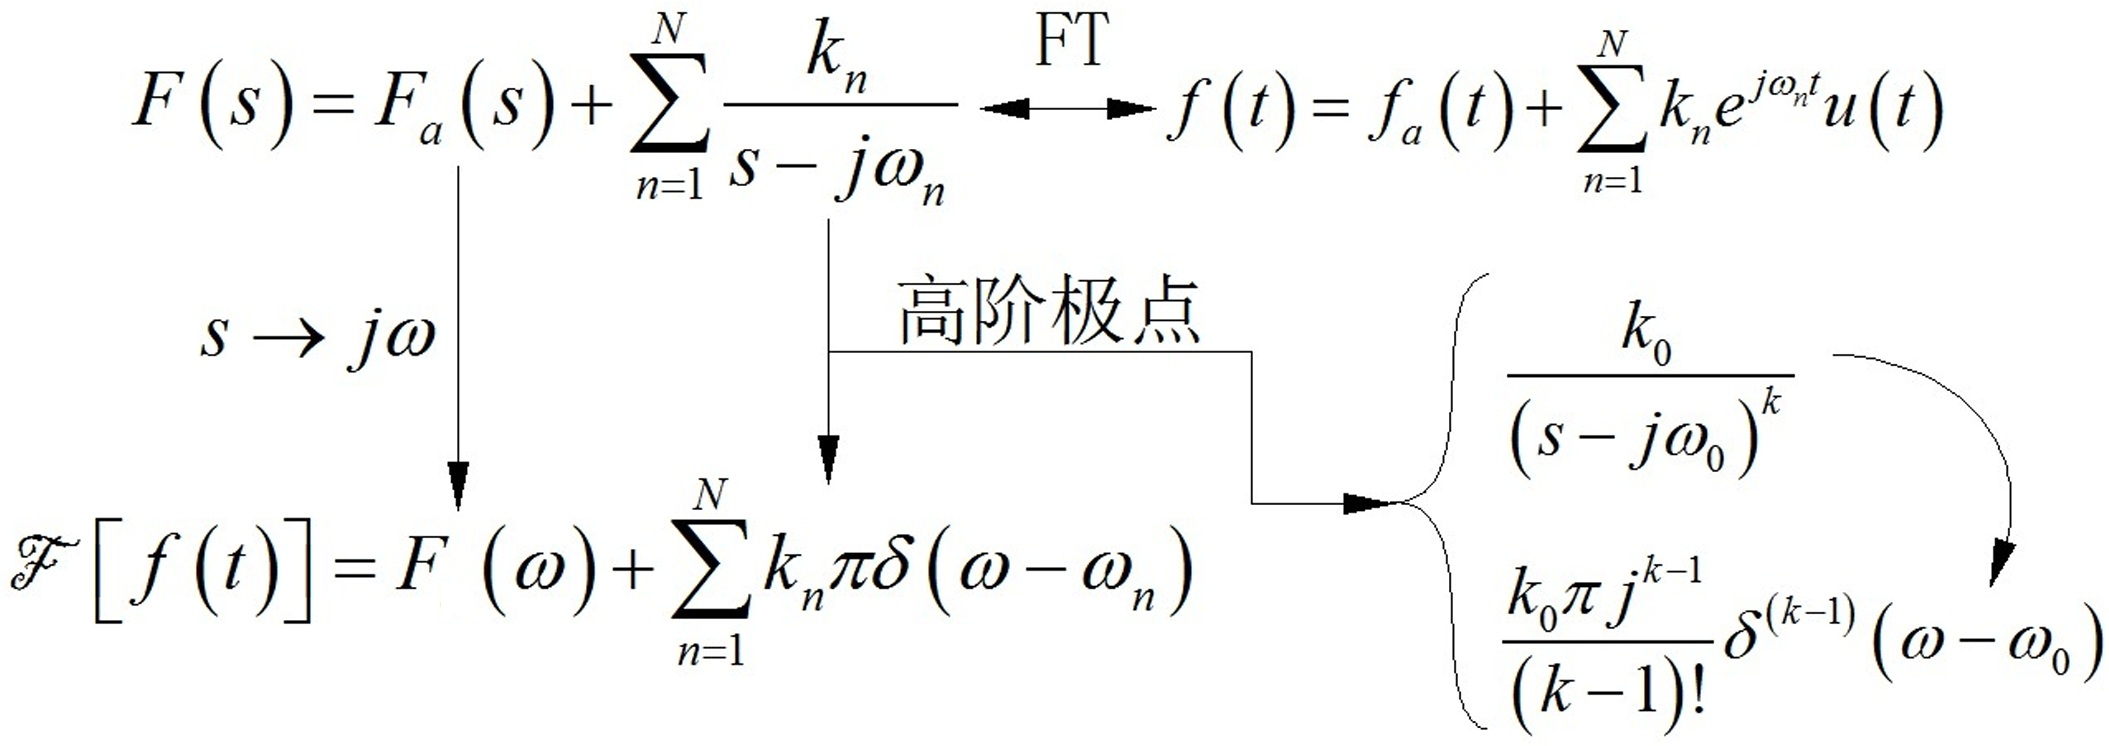
\includegraphics[width=1\linewidth]{image01}
	\label{fig:image01}
\end{figurehere}
\begin{figurehere}
	\centering
	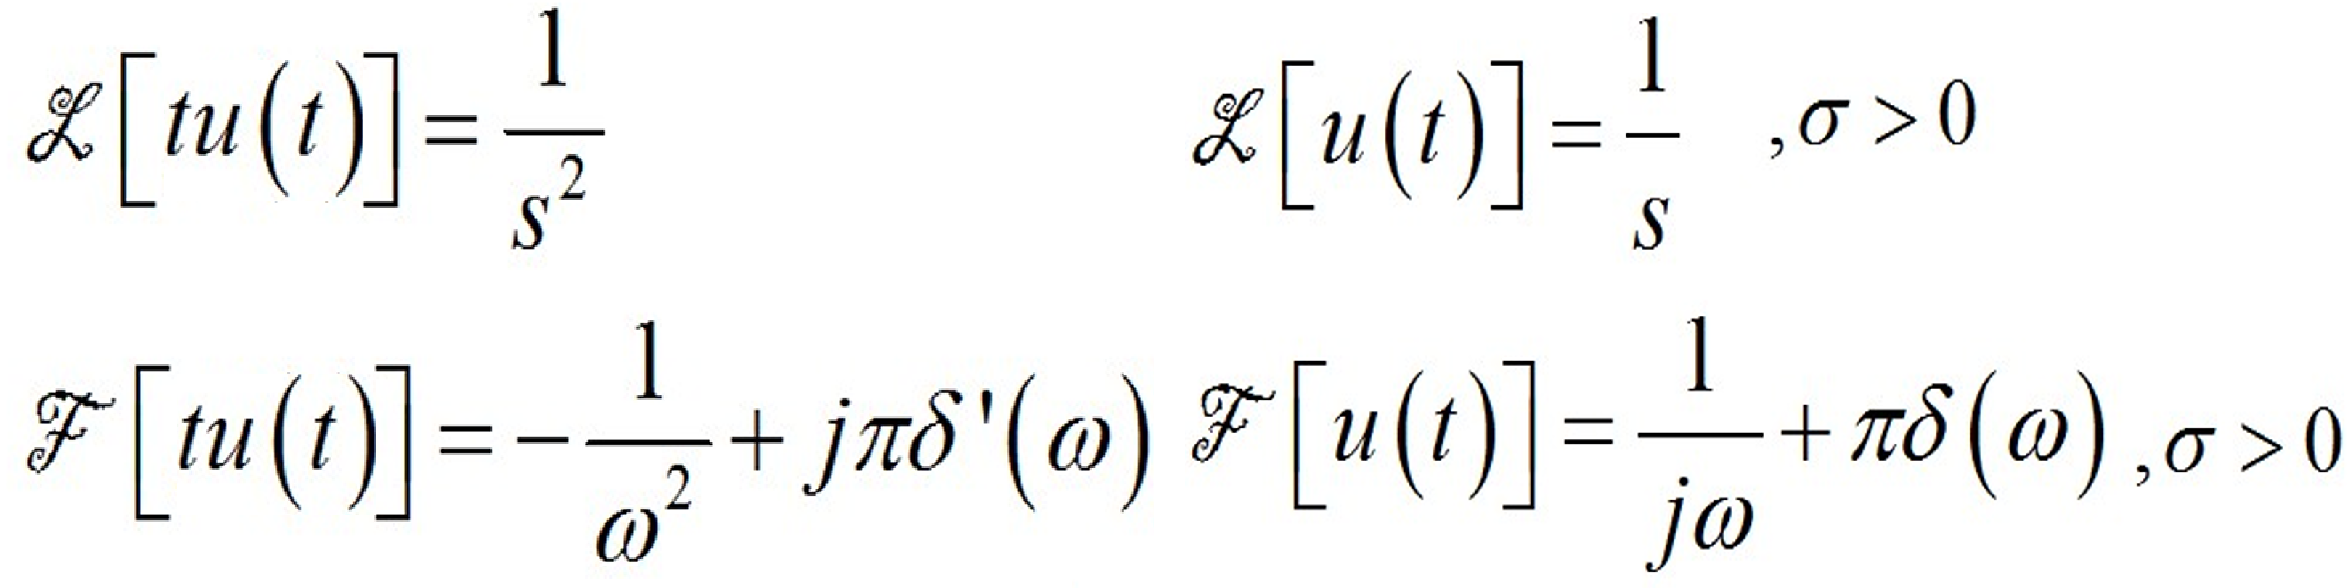
\includegraphics[width=0.95\linewidth]{image02}
	\label{fig:image02}
\end{figurehere}
\textbf{3.ZT到DTFT}

$\begin{cases} \cal{DTFT}[x[n]]=\mathnormal X(e^{j\omega})=\sum\limits_{n=-\infty}^\infty{x[n]e^{-j\omega n}}\\x[n]=\cal{IDTFT}[\mathnormal X(e^{j\omega})]=\frac{1}{2\pi}\int_{-\pi}^{\pi}\mathnormal X(e^{j\omega})e^{j\omega n}d\omega\end{cases}$

性质:把ZT中的z换成$e^{j\omega}$,a换为$e^{j\omega_0}$(频移)

·线性加权:$\cal{DTFT}[x[n]\cdot n]=j\frac{d}{d\omega}X(e^{j\omega})$

·奇偶虚实:$X(e^{j\omega})=X^*(e^{-j\omega})$

·频域卷积:$\cal{DTFT}[x[n]h[n]]=1/2\pi[X(e^{j\omega})*H(e^{j\omega})]$

\section*{六、变换域分析}

用单位样值响应$h[n]$表示LTI的输出:$y[n]\!=\!x[n]\!*\!h[n]$,则离散时间系统的\textbf{传递函数}$H(z)=\tfrac{Y(z)}{X(z)}$

\subsection*{时域特性分析}

·h(t)波形种类仅与极点有关,幅度相角与零极点有关

·极点虚部增加震荡频率增加;极点实部>0指数增加

·h[n]的形式仅与极点有关,幅度相角与零极点有关

·$\omega$增加则震荡频率增加;$r>1$ 指数增加,反之衰减
\begin{center}
\begin{tabularx}{\columnwidth}{|X|p{35pt}|}
	\hline
	\textbf{LT} & \textbf{性质描述} \\ \hline
	原点 $\frac{1}{s} \gets u(t)$  & 常量 \\ \hline
	实数 $\frac{1}{s-a} \gets e^{at}u(t)$ & 指数增/减 \\ \hline
	虚轴共轭 $\frac{w}{s^2+w^2} \gets \sin(wt)u(t)$ & 等幅振荡 \\ \hline
	复共轭 $\frac{w}{(s+a)^2+w^2} \gets e^{-at}\sin(wt)u(t)$ & \tiny{指数增/减振荡} \\ \hline
	原点二重 $\frac{1}{s^2} \gets tu(t)$ & 线性增加 \\ \hline
	实数二重 $\frac{1}{(s+a)^2} \gets te^{-at}u(t)$ &  \\ \hline
	虚轴二重共轭 $\frac{2ws}{(s^2+w^2)^2} \!\gets\! t\sin(wt)u(t)$ &  \\ \hline
\end{tabularx}
\end{center}

$\frac{z}{z-1} \gets u[n]$;$\frac{z}{(z-1)^2}\leftarrow n$;$\frac{z}{z-a} \leftarrow a^n$;$\frac{az}{(z-a)^2}\leftarrow na^n$

\textbf{系统的稳定性}:$h(t)$绝对可积,$h[n]$绝对可和

离散情形:稳定系统H(z)的收敛域必包含单位圆;因果系统H(z)的收敛域包含无穷远(分子阶次小于分母)$\Rightarrow$因果、稳定系统H(z)的\textbf{极点全在单位圆内}

连续:稳定系统H(s)的收敛域必包含虚轴;因果稳定系统H(s)的\textbf{极点均在左半s平面},反因果均在右半

\textbf{Routh判据}:一阶、二阶系统稳定$\Leftrightarrow$特征方程所有系数均为正;三阶系统还要求$a_0a_3>a_1a_2$

\textbf{临界稳定系统}:激励有界时,系统的响应可能有界也可能无界(虚轴上/单位圆上存在一阶极点)

\subsection*{系统频域特性分析}

系统冲激响应的傅里叶变换是系统的频率响应 $H(j\omega)$,系统冲激响应的拉氏变换是系统的系统函数 $H(s)$,在收敛域包括虚轴的稳定系统,有$H(j\omega)=H(s)|_{s=j\omega}$

\textbf{理想低通滤波器}:$H(j\omega)\!=\!e^{-j\omega t_0}$,$|\omega|\!\leq\!\omega_0$;
$|H(j\omega)|$矩形框,$\varphi(j\omega)\!=\!-\omega t_0$,$|\omega|\!\leq\!\omega_0$

1. 单位冲激响应 $h(t)=\frac{\omega_0}{\pi}Sa[\omega_0(t-t_0)]$

2. 单位阶跃响应 $g(t)=\frac{1}{2}+\frac{1}{\pi}Si[\omega_0(t-t_0)]$(9\%过冲)

\textbf{几何确定法}:对于虚轴左侧的零极点(右侧相频相反):

·非常靠近虚轴的极点,附近幅频峰点,相频响应骤减

·非常靠近虚轴的零点,附近幅频下陷,相频响应骤增

·影响程度近大远小

注:对离散时间系统,用$m_o,p_o$分别表示单位圆内外零极点个数,则一个周期内的相位变化$\Delta\varphi|_{\Delta\omega=2\pi}=-2\pi m_o+2\pi p_o$,对于因果稳定系统,有$\Delta\varphi|_{\Delta\omega=2\pi}=-2\pi m_o$

\textbf{全通系统(因果)}:幅频特性为常数、相频特性单调递减;零极点关于虚轴对称/关于单位圆倒共轭分布$z_0\leftrightarrow\frac{1}{z_0^*}$,又由于因果,极点只能在虚轴左侧/单位圆内

\textbf{最小相位系统(因果稳定)}:零点也都位于左半平面/单位圆内(相较于关于虚轴对称到右半平面而言)

·性质:逆系统也是稳定的最小相位系统

·频域特性:与非……相比,幅频一致,相频全程变化最小/单周期变化为0

最小单位系统单位阶跃响应具有负调现象,朝着反方向运动

\textbf{系统的分解}:最小相位系统和全通系统级联(零点去左边,挪回零点)$H(z)\!=\!H_{min}(z)\cdot H_{ap}(z)$

\textbf{负调现象}:非最小相位系统单位阶跃响应一开始向相反方向运动

\begin{figurehere}
	\centering
	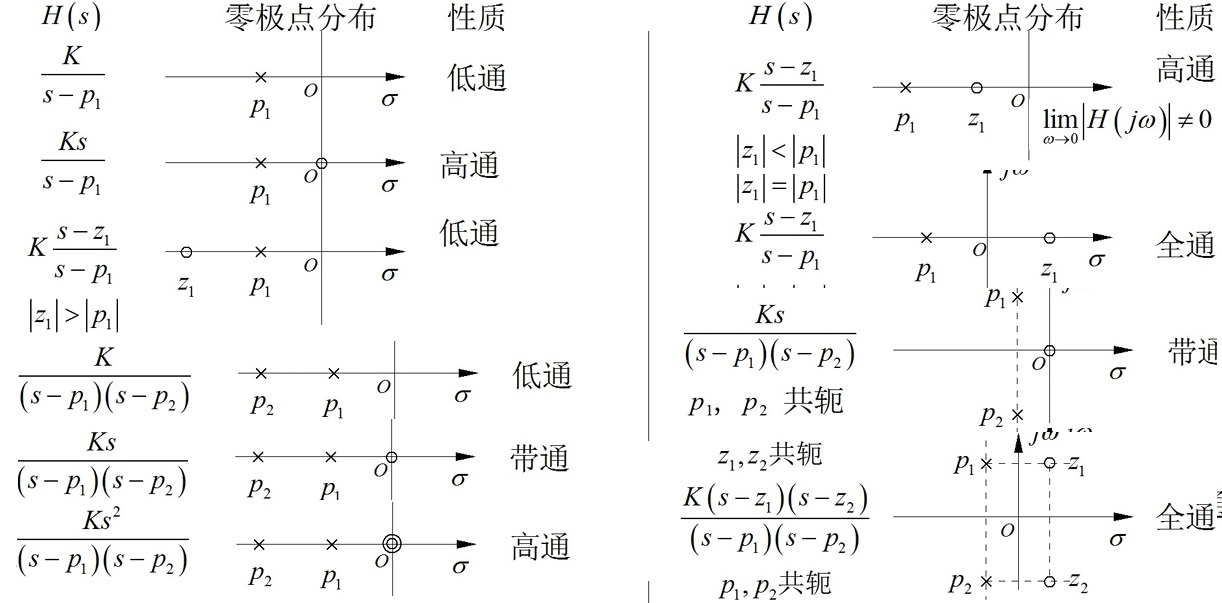
\includegraphics[width=1\linewidth]{image05}
	\label{fig:image05}
\end{figurehere}
\section*{七、DFT系列(信号数值频谱分析)}

\textbf{DFS}:设$x[n]$的周期为N,看成基波$e^{j\frac{2\pi}{N}n}$和各次谐波$e^{j\frac{2\pi}{N}kn}$的线性组合共N个分量(式子见DFT)

\textbf{DFT}:将DFS用于有限长离散时间信号($W\!=\!e^{-j\frac{2\pi}{N}}$)

$DFT[x[n]]={X}[k]=\sum^{N-1}_{n=0} {x}[n] W^{nk} \ \ ,0\leq k\leq N-1$

$IDFT[{X}[k]]\!=\!{x}[n]\!=\!\frac{1}{N}\sum^{N-1}_{k=0} {X}[k] W^{-nk} \ \ ,0\leq n\leq N-1$

\textbf{DFT性质}:

圆移位:有限长序列x[n]圆移位定义为 $f[n]=x((n-m))_NR_N[n]$,其中 $R_N[n]=1,0\leq n\leq N-1$:

·把序列x[n]延拓为周期序列 $x[n] \rightarrow x((n))_N$

·使 $x((n))$沿着n轴移动m位,得到 $x((n-m))_N$,取出上述主值序列

令 $X[k]=DFT[x[n]],\ Y[k]=DFT[y[n]]$,则满足

1. 线性:$DFT[ax[n]+by[n]]=aX[k]+bY[k], \ \forall a,b$

2. 时域圆移位特性:若$f[n]=x((n+m))_NR_N[n], \ x[n]\leftrightarrow X[k]$,则 $F[k]=DFT[f[n]]=W^{-mk}X[k]$

3. 频域圆移位特性:若 $DFT[x[n]]=X[k]$,则 $IDFT[X(k\pm l)_NR_N[k]]=W^{\pm nl}x[n]$

4. 时域圆卷积定理,设 $y[n]\leftrightarrow Y[k], \ x[n]\leftrightarrow X[k], \ f[n]\leftrightarrow F[k]$,若$F[k]=X[k]Y[k]$,则 $f[n]=IDFT[F[k]]=\sum\limits^{N-1}_{m=0} x[m]y((n-m))_NR_N[n]$ ,或$f[n]=\sum\limits^{N-1}_{m=0}y[m]x((n-m))_NR_N[n]$

5. 频域圆卷积,若 $y[n]=x[n]h[n]$,则 $Y[k]=DFT[y[n]]=\frac{1}{N}\sum\limits^{N-1}_{n=0}X[l]H((k-l))_NR_N[k]$ 或 $Y[k]=\frac{1}{N} \sum\limits^{N-1}_{n=0}H[l]X((k-l))_NR_N[k]$

6. 设$x^*[n]$是x[n]的共轭复数序列,则 $DFT[x^*[n]]=X^*[N-k]$
   
   令$X(k)=X_r(k)+jX_i(k)$,则 $X_r(k)=\sum\limits_{n=0}^{N-1}x(n)\cos(\frac{2\pi nk}{N}), \ X_i(k)=-\sum\limits^{N-1}_{n=0}x(n)\sin(\frac{2\pi nk}{N})$

\begin{center}
\begin{tabularx}{\columnwidth}{|c|X|X|X|X|X|X|}
\hline
x[n] & 实函数 & 实偶函数 & 实奇函数 & 虚函数 & 虚偶函数 & 虚奇函数 \\
\hline
X[k] & 实部为偶,虚部为奇 & 实偶函数 & 虚奇函数 & 实部为奇,虚部为偶 & 虚偶函数 & 实奇函数 \\
\hline
\end{tabularx}
\end{center}

7. 帕斯瓦尔定理,$\sum\limits^{N-1}_{n=0}|x[n]|^2=\frac{1}{N}\sum\limits^{N-1}_{k=0}|X[k]|^2$

\subsection*{频率采样理论}

当 $z=W^{-k}=e^{-\frac{2k\pi j}{N}}$ 时,x[n]的Z变换就等于该序列的离散傅里叶变换,即$X[k]=X(z)|_{z=W^{-k}}$

\textbf{频域采样不失真条件}:频域采样点数$N\geq M$序列长度

$X(z)=\sum_{k=0}^{N-1}X[k]\phi_k(z), \phi_k(z)=\frac{1}{N}\frac{1-z^{-N}}{1-W^{-k}z^{-1}}$内插函数,线性相位

\subsection*{FFT计算线卷积方案与复杂度}

DFT 所需复数加法次数 $N^2$, 复数乘法次数 $N(N-1)$;FFT 所需复数加法次数 $N\log_2 N$,复数乘法次数 $\frac{N}{2}\log_2 N$。1次复数乘法相当于4次实数乘法,2次实数加法;一次复数加法相当于2次实数加法。

\textbf{快速卷积方案}:要计算x[n]*h[n],可先将x[n]和h[n]都补零到$N=2^M$长度,分别作FFT得到X(k),H(k),再序列相乘得到X(k)H(k),再对结果进行反傅里叶变换。复数乘法次数:$\frac{3N}{2}\log_2N+N$,即两次FFT+1次IFFT+序列相乘;复数加法次数: $3N\log_2 N$

\textbf{重叠相加法}:分段$x[n]$为长度$m\approx N$,且$m+N-1=2^p$

补零$h[n]$至$m+N-1$,预计算$H[k]=\text{FFT}(h[n])$

每段$x_i[n]$补零至$m+N-1$,计算:$y_i[n]=\text{IFFT}\big(\text{FFT}(x_i[n])\cdot H[k]\big)$

重叠相加:相邻段重叠$N-1$点,对位相加后拼接
\subsection*{用DFT作频谱分析的参数选择与注意问题}

·采样频率$f_s$ 应满足奈奎斯特频率要求 ($\geq 2f_m$ ,其中$f_m$为信号最高频率)

·模拟信号持续时间为 $t_c=NT=N/f_s=1/\Delta f$,其中 $\Delta f$ 为频率分辨率,T为采样间隔;

·考点:DFT点数 $N\geq 2f_m/\Delta f$(通常还要求$N=2^M$)

·栅栏效应,DFT是DTFT $X(e^{j\omega})$的采样,只给出了离散点$\omega=2\pi k/N$的频谱值,而无法得知这些点之间的频谱内容,解决方法:补零技术,在x[n]后面增补若干个零值点

1.混叠效应:时域采样,频域产生周期延拓,当不满足采样定理时会发生频谱混叠,即欠采样现象,此时原来信号的高频分量会形成虚假的低频分量;应提高采样频率/采用抗混叠滤波器(低通,滤除>$1/2\omega_s$部分)

2.频率泄露:对信号进行截取,本质是时域截断,用矩形窗函数作用,截取后的信号频谱的高频段和低频段都会出现波动,并会出现过渡带;应扩大采集信号的时间窗口长度、使用光滑窗口对数据进行平滑

\section*{八、数字滤波器}

\textbf{1. 系统可实现性}
   
佩利—维纳准则:如果系统频率特性平方可积$\int_{-\infty}^{\infty}|H(j\omega)|^2d\omega<\infty$,则$H(j\omega)$物理可实现的必要条件为$\int_{-\infty}^{\infty}{{|ln|H(j\omega)||}\over{1+\omega^2}}d\omega<\infty$

·理想低通、高通、带通、带阻滤波器都不可实现,高斯特性滤波器也不可实现

·某一限定频带内为0——非因果,不可实现

·一般有理多项式构成的幅频特性能满足必要条件,只需判断是否\textbf{平方可积}

·因果系统的系统函数$H(j\omega)=R(\omega)+jX(\omega)$满足希尔伯特变换关系:$R(\omega)={1\over\pi}\int_{-\infty}^{\infty}{{X(\lambda)}\over{\omega-\lambda}}d\lambda$, $X(\omega)=-{1\over\pi}\int_{-\infty}^{\infty}{{R(\lambda)}\over{\omega-\lambda}}d\lambda$

\textbf{2. 无失真传输}
   
系统响应波形与激励波形相同(幅度可以改变),出现时间不同;系统函数:$H(j\omega)=Ke^{-j{\omega}t_0}$;时域恒为常数$K$,频域为过原点的直线(上下移2$k\pi$也等价,别的不行)

失真传输的应用:产生特定波形、产生升余弦信号(取系统的频谱和升余弦信号的频谱相同,可利用窄脉冲产生升余弦信号)、声音合成

·对频带受限的信号,只需考虑频带范围内

·两个无失真系统串联仍无失真,并联可能失真

\textbf{3. 匹配滤波器}

\textbf{定义}:已知输入中可能有信号$s(t)$,能以最低的错误概率判断脉冲$s(t)$的有无的滤波器

\textbf{实际}:根据$s(t)$定制,增强信号分量,减弱噪声分量,满足某一时刻输出端信噪比最大

\textbf{特征}:单位冲激响应:$h(t)=ks(t_m-t)$($s(t)$的反褶),$t_m$为判决时刻,通常取$t_m=T$,$k=1$;实质是接收信号$r(t)=a s(t-t_m)+n_0(t)$与$s(t)$的互相关运算,通过检测相关结果的峰值确定信号延迟以及相应的幅值。

\textbf{应用条件}:已知信号波形$s(t)$;接收信号模型为$r(t)=a s(t-t_m)+n_0(t)$,其中$n_0(t)$为加性白噪声。

*匹配滤波器是线性系统中“最佳”的滤波器(改善信噪比层面)

$s_0(t)=s(t)*h(t)=s(t)*s(T-t)=R_{ss}(t-T)$即$s(t)$的自相关,$R_{ss}(t)=\int_{-\infty}^{\infty}s(\tau)s(t+\tau)d\tau$

应用:雷达测距精度提高——选自相关后形状尖锐的波形(越杂乱的波形通常越好)


\textbf{4. 模拟滤波器}

高频滤波需要模拟滤波器;对于频率重叠的信号滤波可以使用非理想滤波器

\textbf{5. 数字滤波器}
   
·频率特性:$H(e^{j\omega})={\sum_{n=0}^\infty}x[n]e^{-jn\omega}$,具有周期性,关于z对称,模为偶函数,相位是奇函数

·递归式:$y[n]$的表达式中包含$y[n-k]$项

·非递归式:$y[n]$的表达式中不包含$y[n-k]$

·数字滤波器冲激响应分类

~~~~+无限冲激响应(IIR)数字滤波器:递归式,非线性相位

~~~~+有限冲激响应(FIR)数字滤波器:非递归式,线性相位

·区分:$H(z)={{{\sum_{r=0}^M}b_rz^{-r}}\over{1+{\sum_{k=1}^N}a_kz^{-k}}}$,\textbf{若存在$a_k≠0$,构成IIR滤波器;若$a_k$均为0,对应FIR滤波器}

\textbf{IIR结构实现}

·直接型I、II实现:II型也称为典范结构实现,延时单元最少,缺点是要求精度高,调整特性不方便

·级联实现:对系统因式分解,看成递归一阶子系统和递归二阶子系统的级联,也属于最少延时单元实现,便于调整,但乘法次数比直接型多。

·并联实现:对系统部分分式展开,运行速度高,没有运算误差前后级积累,可以单独调整极点,但无法控制零点
\begin{figurehere}
	\centering
	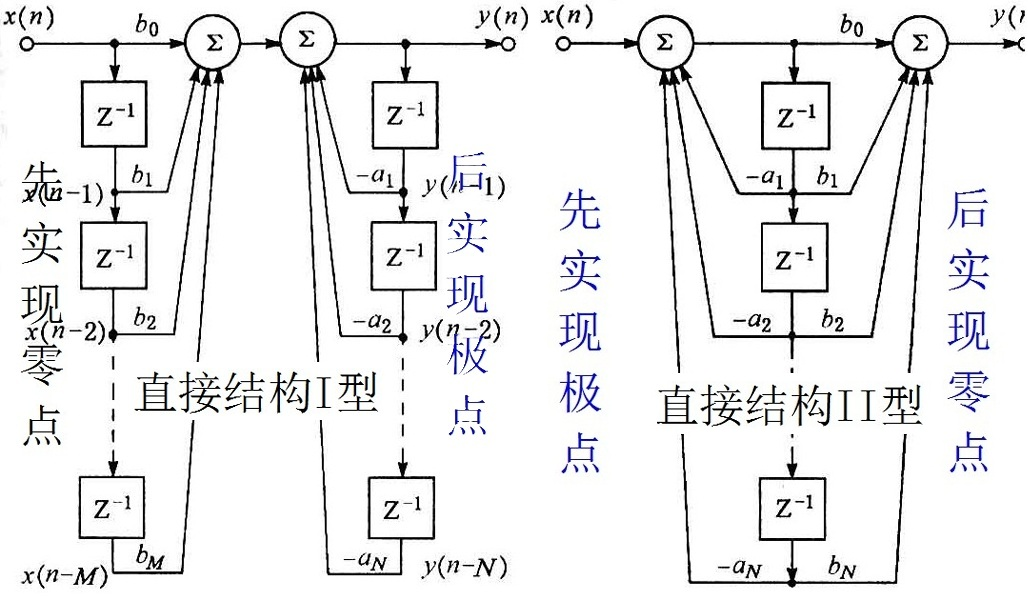
\includegraphics[width=1\linewidth]{image04}
	\label{fig:image04}
\end{figurehere}
\textbf{FIR滤波器特性(FIR是稳定系统)}

·若有限长的实序列$h[n]$满足偶对称($h[n]=h[N-1-n]$)或奇对称($h[n]=-h[N-1-n]$)条件,对应的频率特性具有线性相位。

·$h[n]$偶对称:$H(e^{j\omega})=H_g(\omega)e^{-j\alpha\omega}$,$\alpha={{N-1}\over{2}}$
   
   N为奇数时:$H_g(\omega)$在$\omega=0,\pi,2\pi$偶对称
   
   N为偶数时:$H_g(\omega)$在$\omega=0,2\pi$偶对称,在$\omega=\pi$处奇对称,且$H_g(\pi)=0$,无法实现高通和带阻特性

·$h[n]$奇对称:$H(e^{j\omega})=H_g(\omega)e^{j(\pi/2-\alpha\omega)}$,$\alpha={{N-1}\over{2}}$
   
   N为奇数时:$H_g(\omega)$在$\omega=0,\pi,2\pi$处奇对称,且在这些点$H_g(\omega)=0$,无法实现低通、高通、带阻滤波特性
   
   N为偶数时:$H_g(\omega)$在$\omega=0,2\pi$奇对称,$H_g(0)=0$,无法实现低通、带阻滤波器

\begin{figurehere}
	\centering
	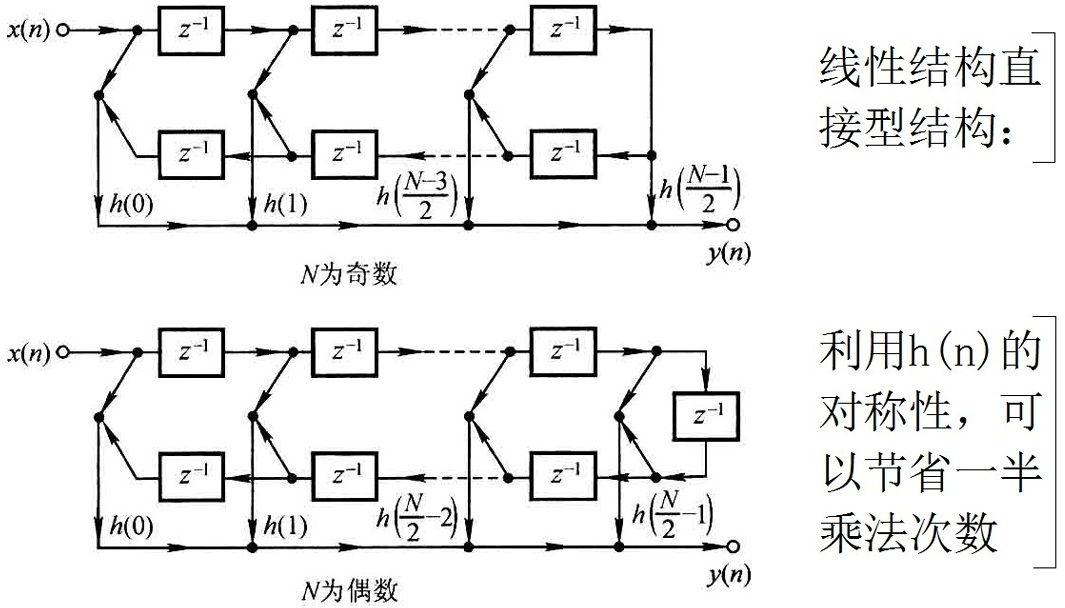
\includegraphics[width=1\linewidth]{image03}
	\label{fig:image03}
\end{figurehere}
\textbf{FIR滤波器设计——窗函数法}

·目标是使设计的滤波器特性$H(e^{j\omega})$与要求的频率特性$H_d(e^{j\omega})$在频域均方误差最小的意义下进行逼近

·矩形加窗对低通滤波器幅频特性影响:频率泄露、形成过渡带、吉布斯现象、负峰影响阻带衰减特性(21dB);增加N可减小过渡带宽度

·窗函数法设计FIR步骤:
   
   由给定$H_d(e^{j\omega})$求出$h_d[n]$,根据通带频率$\omega_p$、截止频率$\omega_s$、衰减要求确定过渡带宽度、窗函数$w[n]$和滤波器长度N,$h[n]=h_d[n]w[n]$。
   
   截止频率$\omega_c=\frac12(\omega_p+\omega_s)$
   
   $N=\frac{2\pi}{\omega_s-\omega_p}×R_\omega$,$R_\omega$为窗函数过渡带宽度系数

\textbf{IIR滤波器设计}

·冲激响应不变法: $H(s)\rightarrow h(t)\rightarrow h[n] \rightarrow H(z)$
   
   模拟滤波器系统函数部分分式展开:$H_a(s)={\sum_{k=1}^N}{{A_k}\over{s-s_k}}$,反拉普拉斯变换得到 $h(t)=\sum^{N}_{k=1}A_ke^{p_kt}u(t)$,采样得到$h[n]=\sum^{N}_{k=1}A_ke^{p_knT}u(nT)$,进行Z变换,得到对应数字滤波器系统函数:$H(z)={\sum_{k=1}^N}{{A_k}\over{1-e^{s_kT}z^{-1}}}$
   
   高频时发生混叠,故只适用于低通、带通滤波器;提高抽样频率可以减少混叠影响。

·双线性变换法
   
   $s=\frac{2}{T}(\frac{1-z^{-1}}{1+z^{-1}})$,$z=\frac{1+(sT/2)}{1-(sT/2)}$
   
   使$s,z$域之间呈单值对应关系,是非线性变换,会引起频率特性失真、相位失真,须作预畸变校正。